\documentclass{article}
\usepackage{graphicx}
\usepackage{hyperref}
\usepackage{textcomp}

\usepackage{xcolor}
\hypersetup{
    colorlinks,
    linkcolor={red!50!black},
    citecolor={blue!50!black},
    urlcolor={blue!80!black}
}
\makeatletter
\g@addto@macro{\UrlBreaks}{\UrlOrds}
\makeatother

\graphicspath{{./pic/}}

\newcommand{\commentJSL}[1]{{\color{cyan} JSL: #1}}
%\color{green}
%\color{mauve}
%\color{blue}

\newcommand{\commentTODO}[1]{{\color{red} #1}}

\newcommand{\stt}[1]{{\small\tt #1}}


%Hide stuff from table of content whiteout loosing numbers
\DeclareRobustCommand{\gobblefour}[5]{} % Use 4 if unremunerated
\newcommand*{\SkipTocEntry}{\addtocontents{toc}{\gobblefour}}

\begin{document}

\title{Getting started with the E-puck}
\author{Johan S. Laursen}

\maketitle
\tableofcontents

\section{Introduction}
This document explains how to get started with remote controlling the e-puck using C++ and the ROS framework. An \textit{e-puck user manual} from AAI Canada is available in the lab. Their manual is a bit dated but gives a detailed introduction to programming the e-puck directly. This document mostly replaces \textit{section 4: Getting Started} of the AAI manual and supplements with updated information and more details regarding how to control the e-puck remotely. The manuals accompanying CD contains useful guides, programs, and c-drivers for the e-puck.

\begin{figure}[h]
\centering
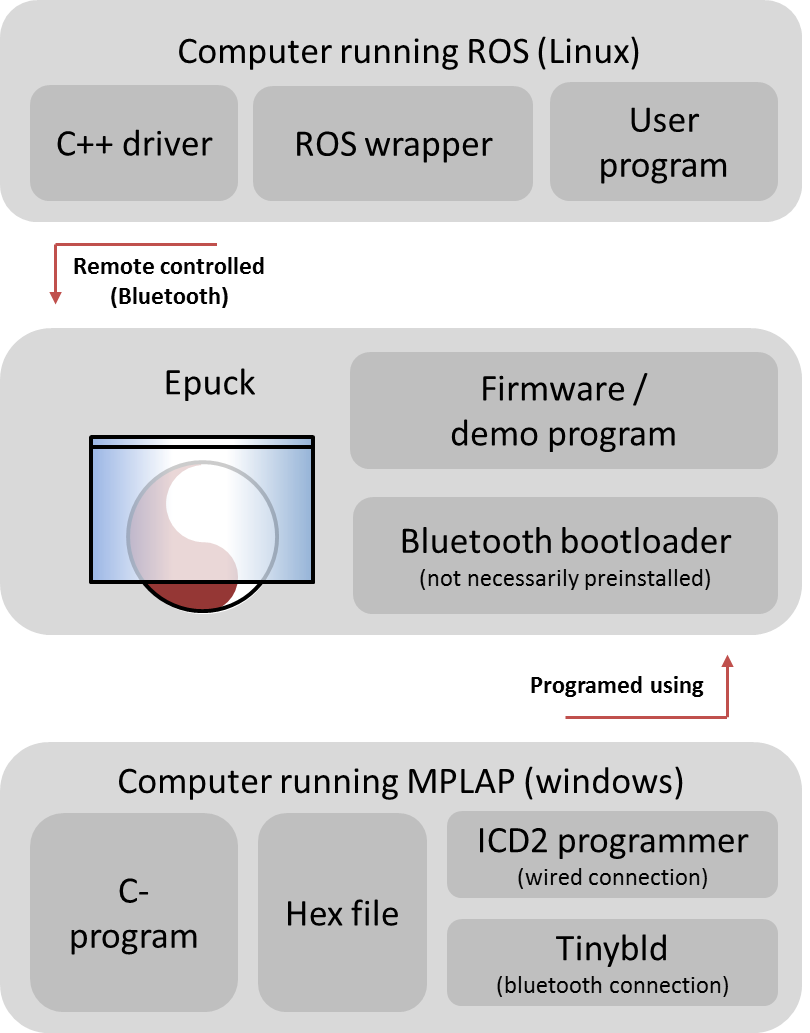
\includegraphics[width=0.6\textwidth]{pipeline}
\caption{Pipeline and overview}
\label{fig:graphexample}
\end{figure}

\subsubsection*{Software currently installed on the e-puck}
In addition to the information regarding the epuck driver this document also gives instructions on how to install both the bluetooth bootloader and the firmware onto the e-puck. This may already be installed onto the epuck depending on how it has been used privously. Likewise the demo program descripbe in AAI canadas manual may not be present on the epuck.

\subsubsection*{The current state of the driver}
A C++ class is used to gain access to the e-pucks sensors and actuators raw values. This is wrapped in ROS for convenience and ROS compliance. This wrapping converts some values into physical units instead of the raw number obtain directly from the e-puck. For instance, using the ROS wrapper speed is given as a linear speed [m/s] and angular speed [rad/s] as opposed to raw integer values. Note that this driver provides a low level interface to the e-puck and does not provide high-level functionality such a tracking, wall-following, point-to-point navigation, etc. Implementation of such can be seen in the reversible e-puck project linked in Sec.~\ref{sec:links}. The code is however not suitable for direct use (as it is only a prototype) but may provide a place for inspiration.  





\newpage
\section{Programming the e-puck}
\subsection{Installing and running MPLAP}

\subsubsection*{Inside the epuck:}
\begin{itemize}
\item Inside the e-puck is a dsPIC30F6014A chipset.
\item This chip is part of 16 bit architecture
\item This chipset is developed by the company Microchip
\end{itemize}

\subsubsection*{Installing the correct Microchip tools}
To transfer compiled programs via cabled to the e-puck requires a proprietary programmer from Microchip and the accompanying toolsuite.
Programmers of type \stt{MPLAB ICD 2} is available in the lab. These programmers are however no longer supported
in newer versions of Microchips programming IDE (MPLAP) and as such older versions of the IDE has to be used. 

The software required to program the e-puck is separated into three parts. 
\begin{itemize}
\item IDE: MPLAP IDE v8.70 \\ (Not to be confused with MPLAP-X which is the newest version)
\item Compiler and chipset specification: MPLAP C30 v3.30b \\ (Found under MPLAB C Compiler for PIC24 and dsPIC DSCs)
\end{itemize}

\subsubsection*{Running MPLAP:}
MPLAP was originally written for Windows XP.  
When running the program enable windows backwards compatibility feature and run the program as an administrator. This is selected by right clicking the icon\textrightarrow properties\textrightarrow compatability.
If the ICD 2 programmer is connected via USB the correct drivers has to be installed (the driver installed automatically by windows does not work).
\footnote{Tested September 2016 using Windows 7 Service Pack 1.}

\subsubsection*{Install the correct ICD 2 USB driver:}
To check the correct driver is installed click:\\
\stt{start -> Computer (right click) -> properties -> device manger}
\\\\\noindent
The driver vertion should be listed as: \\
\stt{Microchip Technology, Inc.}\\
\stt{19-12-2007}\\
\stt{1.0.0.6}
\\\\\noindent
To update the driver click: \\
\stt{Driver tap -> Update driver -> Browse manually -> let me pick from list -> Have disk -> Browse -> <MPLAP IDE folder>/driver64/}
\\\\\noindent
you might have to restart MPLAP and reconnet the programmer after driver changes. 
Also note that the driver used might change depending on which USB port is used. 

\subsubsection*{Install the correct ICD 2 USB driver:}
If a RS232 connection is used to interface with the programmer (using a serial calbel, not the USB cable) the settings for the COM-port has to be modified.
The COM port settings can be edited from the device manger. Follow the instructions in the link and ajust the COM port settings:\\
\url{http://ww1.microchip.com/downloads/en/devicedoc/51265e.pdf}\\
\\\\\noindent
COM Port settings:
\begin{itemize}
 \item Use COM port 1 (MPLAP has truble with higher port numbers)
 \item Set baudrate to 11920
 \item Disable buffer
 \item Set flow to hardware
\end{itemize}

\subsubsection*{Common MPLAP errors:}
Robot is not connected to programmer:\\
\stt{
ICDWarn0020: Invalid target device id (expected=0x2C3, read=0x0)
\\...Reading ICD Product ID
\\Running ICD Self Test
\\... Failed Self Test.}
\\\\\noindent
Incorrect USB driver is used for the ICD 2:\\
\stt{
Connecting to MPLAB ICD 2
\\ICD0019: Communications:  Failed to open port (USB): (Windows::GetLastError() = 0x0, 'The operation completed successfully.')
\\ICD0021: Unable to connect with MPLAB ICD 2 (USB)
\\MPLAB ICD 2 ready for next operation
}



\subsection{Transferring programs via cable}
\label{sec:transfering_cabel}
To install an already compiled program (hex file) on to the e-puck
\begin{enumerate}
\item Open the MPLAP IDE
\item Import the Hex file: 
\\ file \textrightarrow import \textrightarrow  file.hex
\item Connect the programmer: 
\\ programmer\textrightarrow select programmer\textrightarrow  MPLAP ICD 2
\item Transfer the program: 
\\ programmer\textrightarrow Program
\end{enumerate}


\subsection{Transferring programs via Bluetooth}
\subsubsection{Installing the bootloader}
The e-puck does not come with a Bluetooth bootloader preinstalled. However having the bootloader a huge convenience compared to continually unplugging and inserting the programmer.
%
Too install the bootloader:
\begin{enumerate}
\item Download the e-puck software package linked in Sec.~\ref{sec:links} or located on the e-puck support CD
\item Locate the compiled bootloader HEX program
\\ \stt{/tool/bootloader/epuck\_side/tinybld\_ds6014A\_7.37Mhz\_115200uart1\_8xPLL\_with\_LEDs.hex}
\item Transfer the HEX file to the e-puck using cabled approach described in Sec.~\ref{sec:transfering_cabel}.
\end{enumerate}

\subsubsection{using the bootloader in windows}
\begin{enumerate}
\item Install tinyBld linked in Sec.~\ref{sec:links}
\item Browse to the hex file, select the correct COM port and choose a baud rate of 19200Hz. 
\item Click write and hit the reset button on the e-puck 
\end{enumerate}

Tip: \textit{If two new com ports are created during the Bluetooth pairing; the correct port is probably the one with the lowest index of the two.} 

\subsubsection{using the bootloader in unix}
The software package (linked in \ref{sec:link:software}) contains almost the same content as the CD accompanying the manual.
The web-based package also includes small text-based programs which can be used to transfer hex files to the e-puck. 




\newpage
\section{Bluetooth connection to the e-puck}
\subsubsection*{Windows}
In windows this is straight forward.
\begin{enumerate}
\item Use the normal Bluetooth paring process.
\item Select paring based on manually entering the devices paring cod
e\item Use the four digits found in the e-pucks Bluetooth name on the chip beneath the e-pucks extension board
\end{enumerate}

\subsubsection*{Linux}
In Linux paring (for some reason) cannot be done using the normal approach and has to be done using the terminal.
The CD contains both programs and instructions on how to do the paring. Alternatively, the approach described 
in the links section (Sec.~\ref{sec:links}) can be used.













\newpage
\section{Remote controlling the e-puck}
To read and control the e-pucks sensors and actuators remotely requires both an e-puck and computer to 
implementation and run the same interface. Subsection~\ref{sec:driver_epuck_side} deals with the 
driver on the e-puck side while the remaining subsection goes into more details regarding the computer side.


\subsection{The e-puck firmeware}
\label{sec:driver_epuck_side}
Every single firmware implementation, interfaces, or programs for reading and controlling the 
e-puck remotely seems to rely the same interface running on the e-puck.
The interface running on the e-puck is a simple text based UART interface. Multiple implementations of the same interface exist, and as a result there is a lot of precompiled versions and variants of the need firmware can be found ready to be loaded onto the e-puck.
\\
\\A version is located on the CD or inside the git-repository.
\\\stt{/Software/program/BTcom/BTcom.hex}
\\
\\
The most stable version of this firmware is developed by
Cyberbotics for their Webot platform.
The can be found by downloading the trial version of webot in the folder:
\\\stt{/Webots/projects/robots/e-puck/transfer/firmware/firmware-1.5.2.hex}
\\\
\\
\noindent
To install the firmware running on the e-puck side:
\begin{itemize}
\item Locate the hex binary. 
\item Transfer the binaries to the e-puck using one of the methods described previously 
\end{itemize}

\noindent
To confirm the firmware is correctly installed either:
\begin{itemize}
\item Use tinybtl or a similar program and attempt to read and control the robot. (Send 'H' to get menu of commands)
\item Use the test prorgram from the CD or downloaded from \ref{sec:link:software}
\\ \stt{/Software/tool/e-puck\_monitor/EpuckMonitor.exe}
\end{itemize}


\subsection{The computer driver}
The driver on the computer side is an extension and refactoring of the driver ROS C++ driver created by GCtronics.
The driver adds support for controlling the leds on the e-puck using ROS topics and refactors the code
into smaller more manageable pieces making it fairly easy to use the driver without ROS.

\newpage
\subsection{Installing and compiling the driver}
The framework is based on ROS Indigo and uses Linux Bluetooth protocol stack BlueZ. 

To install the framework
\begin{enumerate}
\item Ensure ROS is installed
\item Create or navigate to your catkin\_workspace
\item Checkout the git repository (link~\ref{sec:link:driver}) into the workspace
\item Compile the workspace using \stt{catkin\_make}
\end{enumerate}

\subsection{Launching the driver node}
To lauch the driver:
\begin{enumerate}
\item Find the e-puck number (see AAI manual page 30/31)
\item Find the e-puck mac-address (type \stt{hcitool scan} in terminal)
\item Modify the launch file accordingly \stt{/src/epuck\_driver\_my/launch/epuck.launch}
\item Launch the node \stt{roslaunch epuck\_driver epuck.launch}
\end{enumerate}

\noindent
In addition to the e-puck name and address the launch file also contains several parameters which enables/disables specific sensors and configures the e-puck camera.
\\
\\
To demo the e-puck driver, create a new terminal and type:
\begin{itemize}
\item To run the interface demo node: 
\\\stt{rosrun epuck\_interface\_demo epuck\_interface\_demo} 
\item To view the e-puck camera: 
\\\stt{rosrun image\_view image\_view image:=/camera} 
\item To launch a ros turtle\_sim\_control (manual remote control):
\\\stt{roslaunch epuck\_interface\_demo teleop.launch}
\item To launch Rviz and Gmapping:
\\\stt{roslaunch epuck\_driver gmapping.launch}
\end{itemize}



\subsection{Overview of the driver}
The driver is split into three classes
\begin{itemize}
\item \stt{BluetoothConnection}: Sets up a UART connection the e-puck
\item \stt{BasicCppDriver}: Gives a c++ interface to control the robot
\item \stt{RosWrapper}: Wraps the c++ in a ROS allowing it to run as its own node
\end{itemize}

Inside the GIT-repository hosting the driver is also a package which showcases how it is possible to connect and interface the driver using ROS.

\subsection{The interface}
Communication whith the e-puck is entirely based on ROS topics. The following commands can be useful to obtain information regarding these topics.
\begin{itemize}
\item \stt{rostopic list}
\item \stt{rostopic echo \textless topic name\textgreater}
\item \stt{rostopic info \textless topic name\textgreater}
\end{itemize}

\subsubsection*{Outputs topics}
\begin{itemize}
\item \textbf{proximity: } 
\\Topic name: \stt{/proximityN} 
\\Messeage type: \stt{sensor\_msgs::Range} 
%
\item \textbf{Accelerometer: } 
\\Topic name: \stt{/accel} 
\\Messeage type: \stt{sensor\_msgs::Imu} 
%
\item \textbf{Light: } 
\\Topic name: \stt{/light} 
\\Messeage type: \stt{visualization\_msgs::Marker} 
%
\item \textbf{Motor speed: } 
\\Topic name: \stt{/motor\_speed} 
\\Messeage type: \stt{visualization\_msgs::Marker} 
%
\item \textbf{Selector: } 
\\Topic name: \stt{/selector} 
\\Messeage type: \stt{visualization\_msgs::Marker} 
%
\item \textbf{Microphone: } 
\\Topic name: \stt{/Microphone} 
\\Messeage type: \stt{visualization\_msgs::Marker} 
%
\end{itemize}

\noindent
Information not directly based on robot sensors 
\\ (manily used for integration with other ROS packages ):
\begin{itemize}
\item \textbf{Odomery (calculated based on motor speed): } 
\\Topic name: \stt{/odom} 
\\Messeage type: \stt{nav\_msgs/Odometry} 
%
\item \textbf{Robot transforms: } 
\\Topic name: \stt{/tf} 
\\Messeage type: \stt{tf2\_msgs/TFMessage} 
%
\item \textbf{Laser scan (based on proximity sensor): } 
\\Topic name: \stt{/scan} 
\\Messeage type: \stt{sensor\_msgs/LaserScan} 
\end{itemize}


\subsubsection*{Inputs topics}
\begin{itemize}
\item \textbf{Motor control } 
\\Topic name: \stt{/mobile\_base/cmd\_vel} 
\\Messeage type: \stt{geometry\_msgs::Twist}
\\Format: \stt{Linear speed (msg.linear.x) and angular speed (msg.angular.z)}
%
\item \textbf{Led: } 
\\Topic name: \stt{/leds} 
\\Messeage type: \stt{std\_msgs::UInt32MultiArray} 
\\Format: \stt{Values: 0=off, 1=on, 2=toggle, \\ list[10]=\{led 0, led 1,...,led 7, body led, front led\}}
\end{itemize}





\newpage
\section{Link collection}
\label{sec:links}

\SkipTocEntry
\subsubsection{Genneral information regarding the e-puck:}
\label{sec:link:gen}
\begin{itemize}
\item Official e-puck website: 
\\ \url{http://www.e-puck.org/}
\item GCtronis wiki 
\\ \url{http://www.gctronic.com/doc/index.php/E-Puck}
\end{itemize}

\SkipTocEntry
\subsubsection{Microchip - Tools for programming the e-pucks chipset:}
\label{sec:link:microship}
\begin{itemize}
\item IDE and compiler:
\\ \url{http://www.microchip.com/mplab/mplab-x-ide}
%\item Compiler<>
%\\ \url{http://www.microchip.com/mplab/compilers}
\item Chipset:
\\ \url{http://www.microchip.com/wwwproducts/en/dsPIC30F6014A}
\end{itemize}

\SkipTocEntry
\subsubsection{E-puck software}
\label{sec:link:software}
\begin{itemize}
\item E-puck software 
\\ (E-puck C drivers, Bluetooth bootloader, Linux BT bootloader scrips, etc.)
\\ \url{https://gna.org/svn/?group=e-puck}
\item TinyBootloader 
\\ (GUI program for uploading programs using Bluetooth)
\\ \url{http://www.etc.ugal.ro/cchiculita/software/tinyblddownload.htm}
\item Webot
\\ (Includes the e-puck firmware used for remote-controlling the robot)
\\ \url{https://www.cyberbotics.com/}
\end{itemize}

\SkipTocEntry
\subsubsection{Drivers for remote control of the e-puck:}
\label{sec:link:driver}
\begin{itemize}
\item ROS driver based on C++
\\ (An extension and refactored version of the GCtronics driver linked below) 
\\ \url{https://github.com/skorbiz/epuck_driver}
\end{itemize}


\SkipTocEntry
\subsubsection{Other}
\label{sec:link:other}
\begin{itemize}
\item Info on Bluetooth paring in Linux 
\\ \url{http://www.heatxsink.com/entry/how-to-pair-a-bluetooth-device-from-command-line-on-linux}
\item Reversible e-puck project \\(Inspiration for the implementation of high-level epuck behviours?)
\\ \url{https://github.com/skorbiz/reversible_epuck} 
\end{itemize}


\SkipTocEntry
\subsubsection{Alternative drivers for remote control of the e-puck:}
\label{sec:link:altdrivers}
\begin{itemize}
\item Python driver
\\ \url{http://abitworld.com/projects/epuck-robot-libraries-for-teleoperation/}
\item ROS driver (python based)
\\ \url{https://github.com/verlab-ros-pkg/epuck_driver}
\item ROS driver (Python based, extension of the Verlab driver above)
\\ \url{https://github.com/gctronic/epuck_driver}
\item ROS driver (C++ based, converted version of the GCtronics driver above)
\\ \url{https://github.com/gctronic/epuck_driver_cpp}
\end{itemize}









\end{document}
